\documentclass{ieeetj}
\usepackage{cite}
\usepackage{amsmath,amssymb,amsfonts}
\usepackage{algorithmic}
\usepackage{graphicx,color}
\usepackage{textcomp}
\usepackage{xcolor}
\usepackage{hyperref}
\hypersetup{hidelinks=true}
\usepackage{algorithm,algorithmic}
\def\BibTeX{{\rm B\kern-.05em{\sc i\kern-.025em b}\kern-.08em
    T\kern-.1667em\lower.7ex\hbox{E}\kern-.125emX}}
\AtBeginDocument{\definecolor{tmlcncolor}{cmyk}{0.93,0.59,0.15,0.02}\definecolor{NavyBlue}{RGB}{0,86,125}}




\def\OJlogo{\vspace{-4pt}$<$Society logo(s) and publication title will appear here.$>$}
\def\seclogo{\vspace{10pt}$<$Society logo(s) and publication title will appear here.$>$}

\def\authorrefmark#1{\ensuremath{^{\textbf{#1}}}}

\begin{document}
\receiveddate{XX Month, XXXX}
\reviseddate{XX Month, XXXX}
\accepteddate{XX Month, XXXX}
\publisheddate{XX Month, XXXX}
\currentdate{XX Month, XXXX}
\doiinfo{XXXX.2022.1234567}

\markboth{}{Author {et al.}}

\title{A Review of Traditional Financial Models and Mandelbrotian Alternatives}

\author{Gergely Madarasz, Robert Cserpak, Marton Pall}



\begin{abstract}
Traditional financial models rely on the normal distribution assumption to describe market behavior, yet this foundation is fundamentally flawed. Drawing from Nassim Taleb's\cite{taleb2025} and Benoit Mandelbrot's\cite{mandelbrot2004} works, this paper examines why conventional models like Black-Scholes and the Sharpe ratio fail to capture market realities that consistently exhibit fat tails, asymmetry, and volatility clustering.
We review Mandelbrot's Fractal Market Hypothesis as an alternative, incorporating scaling laws and multifractal properties to model financial markets' complex nature. Combined with Taleb's work on fat-tailed distributions, fractal-based approaches represent a paradigm shift toward more accurate financial modeling with significant implications for risk management and derivative pricing.
\end{abstract}

\begin{IEEEkeywords}
Fractal Market Hypothesis, fat tails, Black-Scholes, financial modeling
\end{IEEEkeywords}

%\IEEEspecialpapernotice{(Invited Paper)}

\maketitle

\section{INTRODUCTION}
\IEEEPARstart{T}{his} document is a template for \LaTeX. If you are
reading a paper or PDF version of this document, please download the
template from the IEEE Web site at 
http://\discretionary{}{}{}ieeeauthorcenter.ieee.org/\discretionary{}{}{}create-your-ieee-article/\discretionary{}{}{}use-authoring-tools-and-ieee-article-templates/\discretionary{}{}{}ieee-article-templates/
so you can use it to prepare your manuscript.
You can also explore using the Overleaf editor at
https://\discretionary{}{}{}www.overleaf.com/\discretionary{}{}{}blog/\discretionary{}{}{}278-how-to-use-overleaf-with-ieee-collabratec-your-quick-guide-to-getting-started\discretionary{}{}{}\#.xsVp6tpPkrKM9

If your paper is intended for a conference, please contact your conference
editor concerning acceptable formats for your particular
conference.

IEEE will do the final formatting of your paper. If your paper is intended
for a conference, please observe the conference page limits.

\subsection{ABBREVIATIONS AND ACRONYMS}
Define abbreviations and acronyms the first time they are used in the text,
even after they have already been defined in the abstract. Abbreviations
such as IEEE, SI, ac, and dc do not have to be defined. Abbreviations that
incorporate periods should not have spaces: write ``C.N.R.S.,'' not ``C. N.
R. S.'' Do not use abbreviations in the title unless they are unavoidable
(for example, ``IEEE'' in the title of this article).

\subsection{OTHER RECOMMENDATIONS}
Use one space after periods and colons. Hyphenate complex modifiers:
``zero-field-cooled magnetization.'' Avoid dangling participles, such as,
``Using (1), the potential was calculated.'' [It is not clear who or what
used (1).] Write instead, ``The potential was calculated by using (1),'' or
``Using (1), we calculated the potential.''

Use a zero before decimal points: ``0.25,'' not ``.25.'' Use ``cm$^3$,'' not
``cc.'' Indicate sample dimensions as ``0.1 cm \texttimes 0.2 cm,'' not
``0.1 \texttimes 0.2 cm$^{2}$.'' The abbreviation for ``seconds'' is ``s,''
not ``sec.'' Use ``Wb/m$^{2}$'' or ``webers per square meter,'' not
``webers/m$^2$.'' When expressing a range of values, write ``7 to 9'' or
``7-9,'' not ``7\textasciitilde 9.''

A parenthetical statement at the end of a sentence is punctuated outside of
the closing parenthesis (like this). (A parenthetical sentence is punctuated
within the parentheses.) In American English, periods and commas are within
quotation marks, like ``this period.'' Other punctuation is ``outside''!
Avoid contractions; for example, write ``do not'' instead of ``don't.'' The
serial comma is preferred: ``A, B, and C'' instead of ``A, B and C.''

If you wish, you may write in the first person singular or plural and use
the active voice (``I observed that \textellipsis'' or ``We observed that \textellipsis''
instead of ``It was observed that \textellipsis''). Remember to check spelling.

Try to avoid using too many typefaces in the same article.
Remember that MathJax cannot handle nonstandard typefaces.

\subsection{EQUATIONS}
To make your equations more
compact, you may use the solidus (~/~), the exp function, or appropriate
exponents. Use parentheses to avoid ambiguities in denominators. Punctuate
equations when they are part of a sentence, as in
\begin{equation}
\label{eq1}
x=\frac{111111111}{12345679}=9 .
\end{equation}
Note that $x$ is math mode because it is a variable.
Be sure that the symbols in your equation have been defined before the
equation appears or immediately following. Italicize symbols ($T$ might refer
to temperature, but T is the unit tesla). Refer to ``(1),'' not ``Eq. (1)''
or ``equation (1),'' except at the beginning of a sentence: ``Equation (1)
is \textellipsis .''

\subsection{Algorithms}
Algorithms should be numbered and include a short title.
They are set off from the text with rules above and below the title and after the last line.
\begin{algorithm}[H]
\caption{Weighted Tanimoto ELM.}\label{alg:alg1}
\begin{algorithmic}
\STATE 
\STATE {\textsc{TRAIN}}$(\mathbf{X} \mathbf{T})$
\STATE \hspace{0.5cm}$ \textbf{select randomly } W \subset \mathbf{X}  $
\STATE \hspace{0.5cm}$ N_\mathbf{t} \gets | \{ i : \mathbf{t}_i = \mathbf{t} \} | $ \textbf{ for } $ \mathbf{t}= -1,+1 $
\STATE \hspace{0.5cm}$ B_i \gets \sqrt{ \textsc{max}(N_{-1},N_{+1}) / N_{\mathbf{t}_i} } $ \textbf{ for } $ i = 1,...,N $
\STATE \hspace{0.5cm}$ \hat{\mathbf{H}} \gets  B \cdot (\mathbf{X}^T\textbf{W})/( \mathbb{1}\mathbf{X} + \mathbb{1}\textbf{W} - \mathbf{X}^T\textbf{W} ) $
\STATE \hspace{0.5cm}$ \beta \gets \left ( I/C + \hat{\mathbf{H}}^T\hat{\mathbf{H}} \right )^{-1}(\hat{\mathbf{H}}^T B\cdot \mathbf{T})  $
\STATE \hspace{0.5cm}\textbf{return} $\textbf{W},  \beta $
\STATE 
\STATE {\textsc{PREDICT}}$(\mathbf{X} )$
\STATE \hspace{0.5cm}$ \mathbf{H} \gets  (\mathbf{X}^T\textbf{W} )/( \mathbb{1}\mathbf{X}  + \mathbb{1}\textbf{W}- \mathbf{X}^T\textbf{W}  ) $
\STATE \hspace{0.5cm}\textbf{return}  $\textsc{sign}( \mathbf{H} \beta )$
\end{algorithmic}
\label{alg1}
\end{algorithm}

\subsection{\LaTeX-SPECIFIC ADVICE}

Please use ``soft'' (e.g., \verb|\eqref{Eq}|) cross references instead
of ``hard'' references (e.g., \verb|(1)|). That will make it possible
to combine sections, add equations, or change the order of figures or
citations without having to go through the file line by line.

Please don't use the \verb|{eqnarray}| equation environment. Use
\verb|{align}| or \verb|{IEEEeqnarray}| instead. The \verb|{eqnarray}|
environment leaves unsightly spaces around relation symbols.

Please note that the \verb|{subequations}| environment in {\LaTeX}
will increment the main equation counter even when there are no
equation numbers displayed. If you forget that, you might write an
article in which the equation numbers skip from (17) to (20), causing
the copy editors to wonder if you've discovered a new method of
counting.

{\BibTeX} gets the bibliographic data from .bib files. If you use {\BibTeX} to produce a
bibliography you must send either the .bbl file or the .bib files.
If you use \texttt{biblatex}, please send the .bib file. The .bbl file
generated by \texttt{biblatex} is not designed to be edited.

If you assign the same label to a
subsubsection and a table, you might find that Table 1 has been cross
referenced as Table IV-B3.

If you put a
\verb|\label| command before the command that updates the counter it's
supposed to be using, the label will pick up the last counter to be
cross referenced instead. In particular, a \verb|\label| command
should not go before the caption of a figure or a table.

Do not use \verb|\nonumber| or \verb|\notag| inside the \verb|{array}| environment. It
will not stop equation numbers inside \verb|{array}| (there won't be
any anyway) and it might stop a wanted equation number in the
surrounding equation.

\section{UNITS}
Use either SI (MKS) or CGS as primary units. (SI units are strongly
encouraged.) English units may be used as secondary units (in parentheses).
This applies to papers in data storage. For example, write ``15 Gb/cm$^{2}$
(100 Gb/in$^{2})$.'' An exception is when English units are used as
identifiers in trade, such as ``3\textonehalf -in disk drive.'' Avoid
combining SI and CGS units, such as current in amperes and magnetic field in
oersteds. This often leads to confusion because equations do not balance
dimensionally. If you must use mixed units, clearly state the units for each
quantity in an equation.

The SI unit for magnetic field strength $H$ is A/m. However, if you wish to use
units of T, either refer to magnetic flux density $B$ or magnetic field
strength symbolized as \textmu $_{0}H$. Use the center dot to separate
compound units, e.g., ``A\textbullet m$^{2}$.''

\section{SOME COMMON MISTAKES}
The word ``data'' is plural, not singular. The subscript for the
permeability of vacuum \textmu $_{0}$ is zero, not a lowercase letter ``o.''
The term for residual magnetization is ``remanence''; the adjective is
``remanent''; do not write ``remnance'' or ``remnant.'' Use the word
``micrometer'' instead of ``micron.'' A graph within a graph is an
``inset,'' not an ``insert.'' The word ``alternatively'' is preferred to the
word ``alternately'' (unless you really mean something that alternates). Use
the word ``whereas'' instead of ``while'' (unless you are referring to
simultaneous events). Do not use the word ``essentially'' to mean
``approximately'' or ``effectively.'' Do not use the word ``issue'' as a
euphemism for ``problem.'' When compositions are not specified, separate
chemical symbols by en-dashes; for example, ``NiMn'' indicates the
intermetallic compound Ni$_{0.5}$Mn$_{0.5}$ whereas ``Ni--Mn'' indicates an
alloy of some composition Ni$_{x}$Mn$_{1-x}$.

Be aware of the different meanings of the homophones ``affect'' (usually a
verb) and ``effect'' (usually a noun), ``complement'' and ``compliment,''
``discreet'' and ``discrete,''
``principal'' (e.g., ``principal investigator'') and ``principle''
(e.g., ``principle of measurement''). Do not confuse ``imply'' and
``infer.''

Prefixes such as ``non,'' ``sub,'' ``micro,'' ``multi,'' and ``ultra'' are
not independent words; they should be joined to the words they modify,
usually without a hyphen. There is no period after the ``et'' in the Latin
abbreviation ``{et al.}'' The abbreviation ``i.e.,'' means
``that is,'' and the abbreviation ``e.g.,'' means ``for example'' (these
abbreviations are not italicized).

IEEE styleguides are available at
https://\discretionary{}{}{}journals.ieeeauthorcenter.ieee.org/\discretionary{}{}{}create-your-ieee-journal-article/\discretionary{}{}{}create-the-text-of-your-article/\discretionary{}{}{}ieee-editorial-style-manual/. {\color{white}{ .}}


\section{GUIDELINES FOR GRAPHICS PREPARATION
AND SUBMISSION}
\subsection{TYPES OF GRAPHICS}
The following list outlines the different types of graphics published in
IEEE journals. They are categorized based on their construction, and use of
color / shades of gray:

\subsubsection{Color/Grayscale Figures}
Figures that are meant to appear in color, or shades of black/gray. Such
figures may include photographs, illustrations, multicolor graphs, and
flowcharts.

\subsubsection{Line Art Figures}
Figures that are composed of only black lines and shapes. These figures
should have no shades or half-tones of gray, only black and white.

\subsubsection{Author Photos}
Head and shoulders shots of authors that appear at the end of our papers.

\subsubsection{Tables}
Data charts which are typically black and white, but sometimes include
color.

\begin{table}
\caption{Units for Magnetic Properties}
\label{table}
\setlength{\tabcolsep}{3pt}
\begin{tabular}{|p{25pt}|p{75pt}|p{115pt}|}
\hline
Symbol&
Quantity&
Conversion from Gaussian and \par CGS EMU to SI $^{\mathrm{a}}$ \\
\hline
$\Phi $&
magnetic flux&
1 Mx $\to  10^{-8}$ Wb $= 10^{-8}$ V$\cdot $s \\
$B$&
magnetic flux density, \par magnetic induction&
1 G $\to  10^{-4}$ T $= 10^{-4}$ Wb/m$^{2}$ \\
$H$&
magnetic field strength&
1 Oe $\to  10^{3}/(4\pi )$ A/m \\
$m$&
magnetic moment&
1 erg/G $=$ 1 emu \par $\to 10^{-3}$ A$\cdot $m$^{2} = 10^{-3}$ J/T \\
$M$&
magnetization&
1 erg/(G$\cdot $cm$^{3}) =$ 1 emu/cm$^{3}$ \par $\to 10^{3}$ A/m \\
4$\pi M$&
magnetization&
1 G $\to  10^{3}/(4\pi )$ A/m \\
$\sigma $&
specific magnetization&
1 erg/(G$\cdot $g) $=$ 1 emu/g $\to $ 1 A$\cdot $m$^{2}$/kg \\
$j$&
magnetic dipole \par moment&
1 erg/G $=$ 1 emu \par $\to 4\pi \times  10^{-10}$ Wb$\cdot $m \\
$J$&
magnetic polarization&
1 erg/(G$\cdot $cm$^{3}) =$ 1 emu/cm$^{3}$ \par $\to 4\pi \times  10^{-4}$ T \\
$\chi , \kappa $&
susceptibility&
1 $\to  4\pi $ \\
$\chi_{\rho }$&
mass susceptibility&
1 cm$^{3}$/g $\to  4\pi \times  10^{-3}$ m$^{3}$/kg \\
$\mu $&
permeability&
1 $\to  4\pi \times  10^{-7}$ H/m \par $= 4\pi \times  10^{-7}$ Wb/(A$\cdot $m) \\
$\mu_{r}$&
relative permeability&
$\mu \to \mu_{r}$ \\
$w, W$&
energy density&
1 erg/cm$^{3} \to  10^{-1}$ J/m$^{3}$ \\
$N, D$&
demagnetizing factor&
1 $\to  1/(4\pi )$ \\
\hline
\multicolumn{3}{p{251pt}}{Vertical lines are optional in tables. Statements that serve as captions for
the entire table do not need footnote letters. }\\
\multicolumn{3}{p{251pt}}{$^{\mathrm{a}}$Gaussian units are the same as cg emu for magnetostatics; Mx
$=$ maxwell, G $=$ gauss, Oe $=$ oersted; Wb $=$ weber, V $=$ volt, s $=$
second, T $=$ tesla, m $=$ meter, A $=$ ampere, J $=$ joule, kg $=$
kilogram, H $=$ henry.}
\end{tabular}
\label{tab1}
\end{table}

\begin{figure}
\centerline{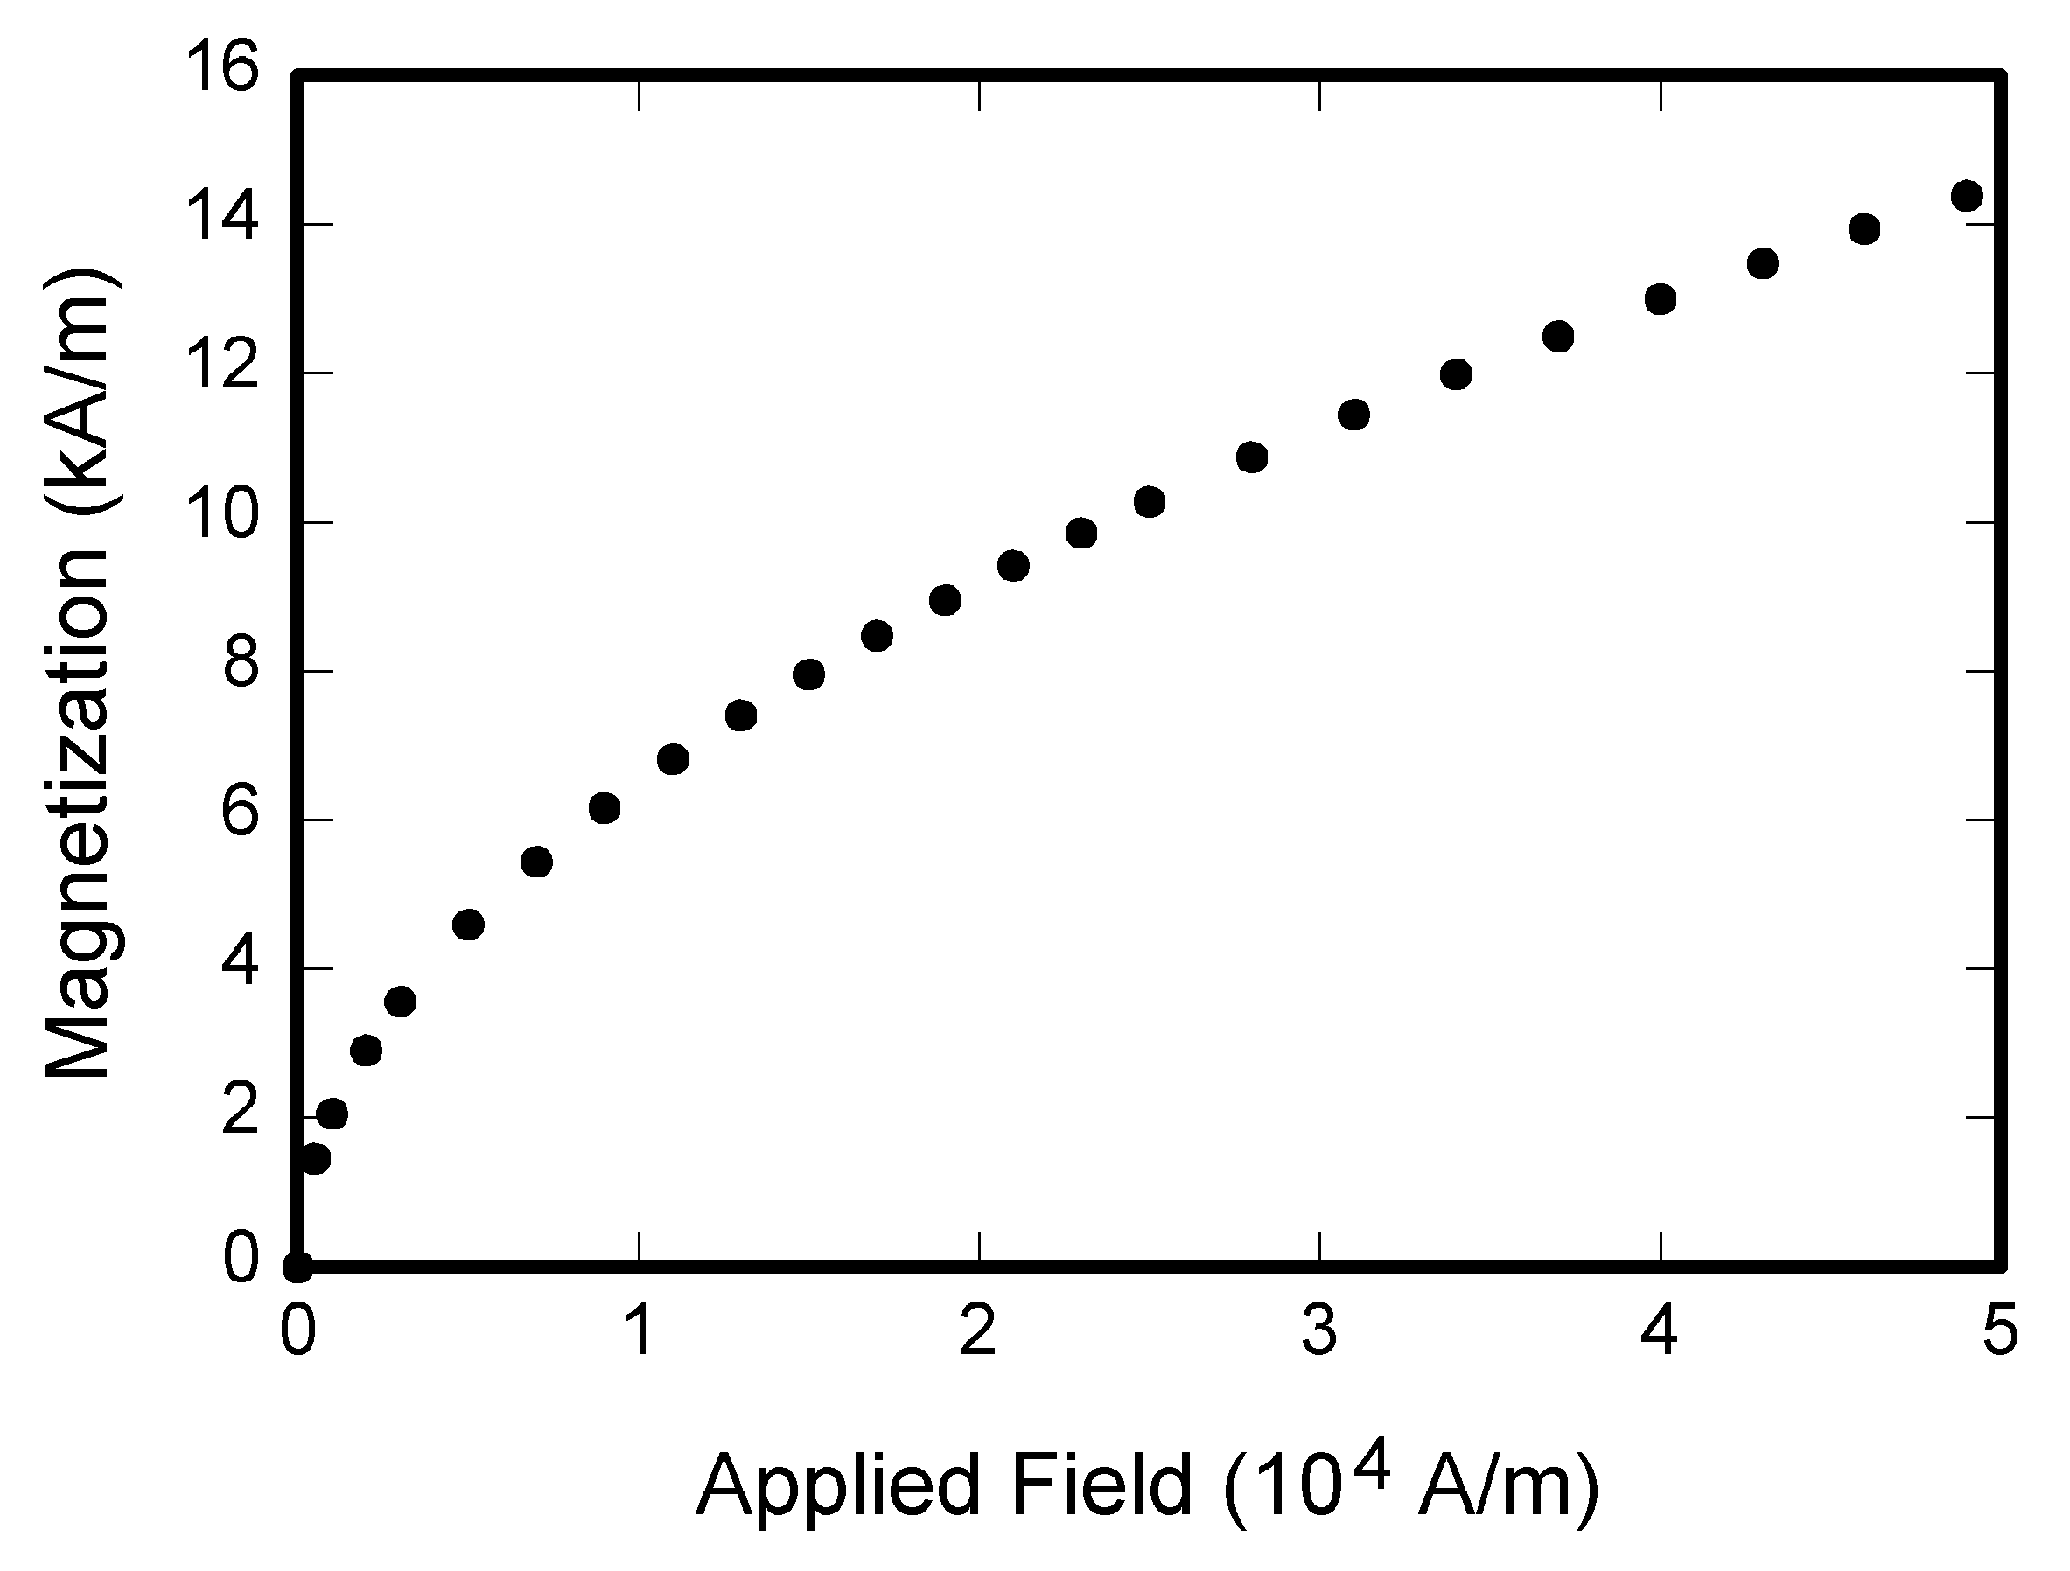
\includegraphics[width=3.5in]{fig1}}
\caption{Magnetization as a function of applied field. 
There is a period after the figure number, followed by two
spaces. It is good practice to explain the significance of the figure in the
caption.\label{fig1}}
\end{figure}

\subsection{MULTIPART FIGURES}
Figures compiled of more than one sub-figure presented side-by-side, or
stacked. If a multipart figure is made up of multiple figure types (one part
is lineart, and another is grayscale or color) the figure should meet the
stricter guidelines.

\subsection{FILE FORMATS FOR GRAPHICS}
Format and save your graphics using a suitable graphics processing program
that will allow you to create the images as PostScript (PS), Encapsulated
PostScript (.EPS), Tagged Image File Format (.TIFF), Portable Document
Format (.PDF), or Portable Network Graphics (.PNG) sizes them, and adjusts
the resolution settings. If you created your source files in one of the
following programs you will be able to submit the graphics without
converting to a PS, EPS, TIFF, PDF, or PNG file: Microsoft Word, Microsoft
PowerPoint, or Microsoft Excel. Though it is not required, it is strongly
recommended that these files be saved in PDF format rather than DOC, XLS, or
PPT. Doing so will protect your figures from common font and arrow stroke
issues that occur when working on the files across multiple platforms. When
submitting your final paper, your graphics should all be submitted
individually in one of these formats along with the manuscript.

\subsection{SIZING OF GRAPHICS}
Most charts, graphs, and tables are one column wide (3.5 inches / 88
millimeters / 21 picas) or page wide (7.16 inches / 181 millimeters / 43
picas). The maximum depth a graphic can be is 8.5 inches (216 millimeters /
54 picas). When choosing the depth of a graphic, please allow space for a
caption. Figures can be sized between column and page widths if the author
chooses, however it is recommended that figures are not sized less than
column width unless when necessary.

The final printed size of author photographs is exactly
1 inch wide by 1.25 inches tall (25.4 millimeters x 31.75 millimeters / 6
picas x 7.5 picas). Author photos printed in editorials measure 1.59 inches
wide by 2 inches tall (40 millimeters x 50 millimeters / 9.5 picas x 12
picas).

\subsection{RESOLUTION}
The proper resolution of your figures will depend on the type of figure it
is as defined in the ``Types of Figures'' section. Author photographs,
color, and grayscale figures should be at least 300dpi. Line art, including
tables should be a minimum of 600dpi.

\subsection{VECTOR ART}
In order to preserve the figures' integrity across multiple computer
platforms, we accept files in the following formats: .EPS/.PDF/.PS. All
fonts must be embedded or text converted to outlines in order to achieve the
best-quality results.

\subsection{COLOR SPACE}
The term color space refers to the entire sum of colors that can be
represented within the said medium. For our purposes, the three main color
spaces are Grayscale, RGB (red/green/blue) and CMYK
(cyan/magenta/yellow/black). RGB is generally used with on-screen graphics,
whereas CMYK is used for printing purposes.

All color figures should be generated in RGB or CMYK color space. Grayscale
images should be submitted in Grayscale color space. Line art may be
provided in grayscale OR bitmap colorspace. Note that ``bitmap colorspace''
and ``bitmap file format'' are not the same thing. When bitmap color space
is selected, .TIF/.TIFF/.PNG are the recommended file formats.

\subsection{ACCEPTED FONTS WITHIN FIGURES}
When preparing your graphics IEEE suggests that you use of one of the
following Open Type fonts: Times New Roman, Helvetica, Arial, Cambria, and
Symbol. If you are supplying EPS, PS, or PDF files all fonts must be
embedded. Some fonts may only be native to your operating system; without
the fonts embedded, parts of the graphic may be distorted or missing.

A safe option when finalizing your figures is to strip out the fonts before
you save the files, creating ``outline'' type. This converts fonts to
artwork what will appear uniformly on any screen.

\subsection{USING LABELS WITHIN FIGURES}
\subsubsection{Figure Axis Labels}
a) Figure axis labels are often a source of confusion. Use words rather than
symbols. As an example, write the quantity ``Magnetization,'' or
``Magnetization $M$,'' not just ``$M$.'' Put units in parentheses. Do not label
axes only with units. As in Figure 1, for example, write ``Magnetization
(A/m)'' or ``Magnetization (A$\cdot $m$^{-1})$,'' not just ``A/m.'' Do not
label axes with a ratio of quantities and units. For example, write
``Temperature (K),'' not ``Temperature/K.''

b) Multipliers can be especially confusing. Write ``Magnetization (kA/m)'' or
``Magnetization (10$^{3}$ A/m).'' Do not write ``Magnetization (A/m)
\texttimes 1000'' because the reader would not know whether the top axis
label in Figure 1 meant 16000 A/m or 0.016 A/m. Figure labels should be
legible, approximately 8 to 10 point type.

\subsubsection{Subfigure Labels in Multipart Figures and Tables}
Multipart figures should be combined and labeled before final submission.
Labels should appear centered below each subfigure in 8 point Times New
Roman font in the format of (a) (b) (c).

\subsection{FILE NAMING}
Figures (line artwork or photographs) should be named starting with the
first 5 letters of the author's last name. The next characters in the
filename should be the number that represents the sequential location of
this image in your article. For example, in author ``Anderson's'' paper, the
first three figures would be named ander1.tif, ander2.tif, and ander3.ps.

Tables should contain only the body of the table (not the caption) and
should be named similarly to figures, except that ``.t'' is inserted
in-between the author's name and the table number. For example, author
Anderson's first three tables would be named ander.t1.tif, ander.t2.ps,
ander.t3.eps.

Author photographs should be named using the first five characters of the
pictured author's last name. For example, four author photographs for a
paper may be named: oppen.ps, moshc.tif, chen.eps, and duran.pdf.

If two authors or more have the same last name, their first initial(s) can
be substituted for the fifth, fourth, third\textellipsis letters of their surname
until the degree where there is differentiation. For example, two authors
Michael and Monica Oppenheimer's photos would be named oppmi.tif, and
oppmo.eps.

\subsection{REFERENCING A FIGURE OR TABLE WITHIN YOUR PAPER}
When referencing your figures and tables within your paper, use Figure
and Table. Do not abbreviate. Tables should be numbered with Arabic Numerals.

\subsection{SUBMITTING YOUR GRAPHICS}
Because IEEE will do the final formatting of your paper,
you do not need to position figures and tables at the top and bottom of each
column. In fact, all figures, figure captions, and tables can be placed at
the end of your paper. In addition to, or even in lieu of submitting figures
within your final manuscript, figures should be submitted individually,
separate from the manuscript in one of the file formats listed above in
Section VI-J. Place figure captions below the figures; place table titles
above the tables. Please do not include captions as part of the figures, or
put them in ``text boxes'' linked to the figures. Also, do not place borders
around the outside of your figures.

\subsection{COLOR PROCESSING / PRINTING IN IEEE JOURNALS}
Electronically published journals allow authors to use color without extra charge.
For journals that will print, the charge for print color is \$275 per color figure.
Figures for print journals will otherwise appear in color online, black and white in print (free, no charge).

\section{CONCLUSION}
A conclusion section is not required. Although a conclusion may review the
main points of the paper, do not replicate the abstract as the conclusion. A
conclusion might elaborate on the importance of the work or suggest
applications and extensions.

\section*{APPENDIX}
Appendixes, if needed, appear before the acknowledgment.

\section*{REFERENCES AND FOOTNOTES}
\subsection{REFERENCES}
References need not be cited in text. When they are, they appear on the
line, in square brackets, inside the punctuation. Multiple references are
each numbered with separate brackets. When citing a section in a book,
please give the relevant page numbers. In text, refer simply to the
reference number. Do not use ``Ref.'' or ``reference'' except at the
beginning of a sentence: ``Reference [3] shows \textellipsis .'' Please do not use
automatic endnotes in \textit{Word}, rather, type the reference list at the end of the
paper using the ``References'' style.

Reference numbers are set flush left and form a column of their own, hanging
out beyond the body of the reference. The reference numbers are on the line,
enclosed in square brackets. In all references, the given name of the author
or editor is abbreviated to the initial only and precedes the last name. Use
them all; use \textit{et al}.\ only if names are not given.
Abbreviate conference titles. When citing IEEE Transactions,
provide the issue number, page range, volume number, year, and/or month if
available. When referencing a patent, provide the day and the month of
issue, or application. References may not include all information; please
obtain and include relevant information. Do not combine references. There
must be only one reference with each number. If there is a URL included with
the print reference, it can be included at the end of the reference.

Other than books, capitalize only the first word in a paper title, except
for proper nouns and element symbols. For papers published in translation
journals, please give the English citation first, followed by the original
foreign-language citation. See the end of this document for formats and
examples of common references. For a complete discussion of references and
their formats, see the IEEE style manual at 
https://\discretionary{}{}{}journals.ieeeauthorcenter.ieee.org/\discretionary{}{}{}create-your-ieee-journal-article/\discretionary{}{}{}create-the-text-of-your-article/\discretionary{}{}{}ieee-editorial-style-manual/.


\subsection{FOOTNOTES}
Number footnotes separately in superscripts (Insert\textbar
Footnote).\footnote{It is recommended that footnotes be avoided. Instead,
try to integrate the footnote information into the text.} Place the actual
footnote at the bottom of the column in which it is cited; do not put
footnotes in the reference list (endnotes). Use letters for table footnotes
(see Table 1).

\section{SUBMITTING YOUR PAPER FOR REVIEW}

\subsection{REVIEW STAGE USING SCHOLARONE MANUSCRIPTS}

Contributions to the Transactions, Journals, and Letters may be submitted electronically on IEEE's online manuscript submission and peer-review system, ScholarOne Manuscripts. You can get help choosing the correct publication for your manuscript as well as find their corresponding ScholarOne Manuscripts peer review site using the tools listed at http://\discretionary{}{}{}www.ieee.org/\discretionary{}{}{}publications\_standards/\discretionary{}{}{}publications/\discretionary{}{}{}authors/\discretionary{}{}{}authors\_submission.html. Once you have chosen your publication and navigated to the ScholarOne site, check first to see if you have an existing account. If there is none, please create a new account. After logging in, go to your Author Center and click ``Start New Submission.''

Along with other information, you will be asked to select the manuscript type from the journal's pre-determined list of options. Depending on the journal, there are various steps to the submission process; please make sure to carefully answer all of the submission questions presented to you. At the end of each step you must click ``Save and Continue''; just uploading the paper is not sufficient. After the last step, you should see a confirmation that the submission is complete. You should also receive an e-mail confirmation. For inquiries regarding the submission of your paper on ScholarOne Manuscripts, please contact oprs-support@ieee.org or call +1 732 465 5861.

ScholarOne Manuscripts will accept files for review in various formats. There is a ``Journal Home'' link on the log-in page of each ScholarOne Manuscripts site that will bring you to the journal's homepage with their detailed requirements; please check these guidelines for your particular journal before you submit.

\subsection{FINAL STAGE USING SCHOLARONE MANUSCRIPTS}
Upon acceptance, you will receive an email with specific instructions regarding the submission of your final files. To avoid any delays in publication, please be sure to follow these instructions. Final submissions should include source files of your accepted manuscript, high quality graphic files (if not embedded in your source file), and a formatted pdf file. The accepted version of your manuscript will also be sent to the IEEE publication teams for a comparison to the final files to ensure no significant or unauthorized changes were made after acceptance. If you have any questions regarding the final submission process, please contact the administrative contact for the journal. 

When submitting your final files on a hybrid OA journal you will have the opportunity to designate your article as ``open access'' if you agree to pay the IEEE open access fee. Please select the appropriate choice. Immediately after you have submitted your final files through ScholarOne Manuscripts you will be automatically redirected to the IEEE electronic copyright form wizard. Please complete the copyright at that time to avoid publication delays. 

\subsection{COPYRIGHT FORM}
\looseness1Authors must submit an electronic IEEE Copyright Form (eCF) upon submitting
their final manuscript files. You can access the eCF system through your
manuscript submission system or through the Author Gateway. You are
responsible for obtaining any necessary approvals and/or security
clearances. For additional information on intellectual property rights,
visit the IEEE Intellectual Property Rights department web page at
https://\discretionary{}{}{}www.ieee.org/\discretionary{}{}{}publications/\discretionary{}{}{}rights/\discretionary{}{}{}index.html.

\section{IEEE GUIDELINES AND POLICIES}

A full overview of IEEE publishing guidelines and policies can be found at https://journals.ieeeauthorcenter.ieee.org/become-an-ieee-journal-author/publishing-ethics/guidelines-and-policies/. They are designed to help authors understand and navigate the publishing process successfully. Learn more about IEEE's fundamental publishing guidelines and principles, submission and peer review policies, post-publication policies, and guidelines on advertising, accessibility, and data privacy.

\section*{ACKNOWLEDGMENT}
The preferred spelling of the word ``acknowledgment'' in
American English is without an ``e'' after the ``g.'' Use the
singular heading even if you have many acknowledgments.
Avoid expressions such as ``One of us (S.B.A.) would like
to thank . . . .'' Instead, write ``F. A. Author thanks . . . .'' In
most cases, sponsor and financial support acknowledgments
are placed in the unnumbered footnote on the first page, not
here.

\section*{REFERENCES}

\def\refname{\vadjust{\vspace*{-2.5em}}} %Please don't do this in a real paper.

\noindent\textit{Basic format for books:}

\noindent J. K. Author, ``Title of chapter in the book,'' in {\it Title of His Published Book, x}th ed. City of Publisher,
(only U.S. State), Country: Abbrev. of Publisher, year, ch. $x$, sec. $x$,\break pp.~{\it xxx--xxx.}

{\it Examples:}

\begin{thebibliography}{00}\leftskip1pc\leftskip1pc
\bibitem{bib1} G. O. Young, ``Synthetic structure of industrial plastics,'' in {\it Plastics,}2$^{\mathrm{nd}}$ ed., vol. 3, J. Peters, Ed. New York, NY, USA: McGraw-Hill, 1964, pp. 15--64.
\bibitem{bib2} W.-K. Chen, {\it Linear Networks and Systems.}Belmont, CA, USA: Wadsworth, 1993, pp. 123--135.
\end{thebibliography}

\noindent {\it Basic format for periodicals:}

\noindent J. K. Author, ``Name of paper,'' {\it Abbrev. Title of Periodical}, vol. {\it x, no}. $x, $pp{\it . xxx-xxx,}Abbrev. Month, year, DOI.
 {10.1109.} {{\it XXX}} {.123456}.

{\it Examples:}

\begin{thebibliography}{00}\leftskip1pc
\bibitem{bib3} J. U. Duncombe, ``Infrared navigation---Part I: An assessment of feasibility,'' {\it IEEE Trans. Electron Devices}, vol. ED-11, no. 1, pp. 34--39, Jan. 1959, doi:.  {10.1109/TED.2016.2628402}.
\bibitem{bib4} E. P. Wigner, ``Theory of traveling-wave optical laser,''
{\it Phys. Rev}., vol. 134, pp. A635--A646, Dec. 1965, doi:  {10.1109.} {{\it XXX}} {.123456}.
\bibitem{bib5} E. H. Miller, ``A note on reflector arrays,'' {\it IEEE Trans. Antennas Propagat}., to be published.
\end{thebibliography}

\noindent {\it Basic format for reports:}

\noindent J. K. Author, ``Title of report,'' Abbrev. Name of Co., City of Co., Abbrev.
State, Country, Rep. {\it xxx}, year.

{\it Examples:}

\begin{thebibliography}{00}\leftskip1pc
\bibitem{bib6} E. E. Reber, R. L. Michell, and C. J. Carter, ``Oxygen absorption in the earth's atmosphere,'' Aerospace Corp., Los Angeles, CA, USA, Tech. Rep. TR-0200 (4230-46)-3, Nov. 1988.
\bibitem{bib7} J. H. Davis and J. R. Cogdell, ``Calibration program for the 16-foot antenna,'' Elect. Eng. Res. Lab., Univ. Texas, Austin, TX, USA, Tech. Memo. NGL-006-69-3, Nov. 15, 1987.
\end{thebibliography}

\noindent {\it Basic format for handbooks:}

\noindent {\it Name of Manual/Handbook, x} ed., Abbrev. Name of Co., City of Co., Abbrev. State, Country, year, pp.
{\it xxx-xxx.}

{\it Examples:}

\begin{thebibliography}{00}\leftskip1pc
\bibitem{bib8} {\it Transmission Systems for Communications}, 3rd ed., Western Electric Co., Winston-Salem, NC, USA, 1985, pp. 44--60.
\bibitem{bib9} {\it Motorola Semiconductor Data Manual}, Motorola Semiconductor Products Inc., Phoenix, AZ, USA, 1989.
\end{thebibliography}

\noindent {\it Basic format for books (when available online):}

\noindent J. K. Author, ``Title of chapter in the book,'' in {\it Title of Published Book}, $x$th ed. City of
Publisher, State, Country: Abbrev. of Publisher, year, ch.$x$, sec. $x$, pp.
{\it xxx--xxx}. [Online]. Available:  {http://www.web.com}




{\it Examples:}

\begin{thebibliography}{00}\leftskip1pc
\bibitem{bib10} G. O. Young, ``Synthetic structure of industrial plastics,'' in Plastics, vol. 3, Polymers of Hexadromicon, J. Peters, Ed., 2nd ed. New York, NY, USA: McGraw-Hill, 1964, pp. 15-64. [Online]. Available:  {http://www.bookref.com}.
\bibitem{bib11} {\it The Founders' Constitution}, Philip B. Kurland and Ralph Lerner, eds., Chicago, IL, USA: Univ. Chicago Press, 1987. [Online]. Available:  {http://press-pubs.uchicago.edu/founders/}
\bibitem{bib12} The Terahertz Wave eBook. ZOmega Terahertz Corp., 2014. [Online]. Available:  {http://dl.z-thz.com/eBook/zomega\_ebook\_pdf\_1206\_sr.pdf}. Accessed on: May 19, 2014.
\bibitem{bib13} Philip B. Kurland and Ralph Lerner, eds., {\it The Founders' Constitution.}Chicago, IL, USA: Univ. of Chicago Press, 1987, Accessed on: Feb. 28, 2010, [Online] Available:  {http://press-pubs.uchicago.edu/founders/}
\end{thebibliography}

\noindent {\it Basic format for journals (when available online):}

\noindent J. K. Author, ``Name of paper,'' {\it Abbrev. Title of Periodical}, vol. $x$, no. $x$, pp. {\it xxx-xxx}, Abbrev. Month, year.
Accessed on: Month, Day, year, doi:  {10.1109.} {{\it
XXX}} {.123456}, [Online].

{\it Examples:}

\begin{thebibliography}{00}\leftskip1pc
\bibitem{bib14} J. S. Turner, ``New directions in communications,'' {\it IEEE J. Sel. Areas Commun}., vol. 13, no. 1, pp. 11-23, Jan. 1995. DOI.  {10.1109.} {{\it XXX}} {.123456}.
\bibitem{bib15} W. P. Risk, G. S. Kino, and H. J. Shaw, ``Fiber-optic frequency shifter using a surface acoustic wave incident at an oblique angle,'' {\it Opt. Lett.}, vol. 11, no. 2, pp. 115--117, Feb. 1986, doi: {10.1109.} {{\it XXX}} {.123456}.
\bibitem{bib16} P. Kopyt {\it \textit{et al.}, ``}Electric properties of graphene-based conductive layers from DC up to terahertz range,'' {\it IEEE THz Sci. Technol.,}to be published, doi:  {10.1109/TTHZ.2016.2544142}.
\end{thebibliography}

\noindent {\it Basic format for papers presented at conferences (when available online):}

\noindent J.K. Author. (year, month). Title. presented at abbrev. conference title.
[Type of Medium]. Available: site/path/file

{\it Example:}

\begin{thebibliography}{00}\leftskip1pc
\bibitem{bib17} PROCESS Corporation, Boston, MA, USA. Intranets: Internet technologies deployed behind the firewall for corporate productivity. Presented at INET96 Annual Meeting. [Online]. Available:  {http://home.process.com/Intranets/wp2.htp}
\end{thebibliography}

\noindent {\it Basic format for reports and handbooks (when available online):}

\noindent J. K. Author. ``Title of report,'' Company. City, State, Country. Rep. no.,
(optional: vol./issue), Date. [Online] Available:
{site/path/file}

{\it Examples:}

\begin{thebibliography}{00}\leftskip1pc
\bibitem{bib18} R. J. Hijmans and J. van Etten, ``Raster: Geographic analysis and modeling with raster data,'' R Package Version 2.0-12, Jan. 12, 2012. [Online]. Available:  {http://CRAN.R-project.org/package$=$raster} {}
\bibitem{bib19} Teralyzer. Lytera UG, Kirchhain, Germany [Online]. Available: http://www.lytera.de/Terahertz\_THz\_Spectroscopy.php?id$=$home, Accessed on: Jun. 5, 2014
\end{thebibliography}

\noindent {\it Basic format for computer programs and electronic documents (when available online):}

\noindent Legislative body. Number of Congress, Session. (year, month day). {\it Number of bill or resolution}, {\it Title}. [Type
of medium]. Available: site/path/file

\noindent {\bf {\it NOTE:}} ISO recommends that capitalization follow the accepted
practice for the language or script in which the information is given.



{\it Example:}

\begin{thebibliography}{00}\leftskip1pc
\bibitem{bib20} U.S. House. 102nd Congress, 1st Session. (1991, Jan. 11). {\it H. Con. Res. 1, Sense of the Congress on Approval of Military Action}. [Online]. Available: LEXIS Library: GENFED File: BILLS
\end{thebibliography}

\noindent {\it Basic format for patents (when available online):}

\noindent Name of the invention, by inventor's name. (year, month day). Patent Number  [Type
of medium]. Available:  {site/path/file}

{\it Example:}

\begin{thebibliography}{00}\leftskip1pc
\bibitem{bib21} Musical toothbrush with mirror, by L.M.R. Brooks. (1992, May 19). Patent D 326 189 [Online]. Available: NEXIS Library: LEXPAT File: DES
\end{thebibliography}


\noindent {\it Basic format for conference proceedings (published):}

\noindent J. K. Author, ``Title of paper,'' in {\it Abbreviated Name of Conf.}, City of Conf., Abbrev. State (if
given), Country, year, pp. {\it xxxxxx.}

{\it Example:}

\begin{thebibliography}{00}\leftskip1pc
\bibitem{bib22} D. B. Payne and J. R. Stern, ``Wavelength-switched passively coupled single-mode optical network,'' in {\it Proc. IOOC-ECOC,}Boston, MA, USA,  1985,
pp. 585--590, doi:  {10.1109.} {{\it XXX}} {.123456}.
\end{thebibliography}

{\it Example for papers presented at conferences (unpublished):}

\begin{thebibliography}{00}\leftskip1pc
\bibitem{bib23} D. Ebehard and E. Voges, ``Digital single sideband detection for interferometric sensors,'' presented at the {\it 2nd Int. Conf. Optical Fiber Sensors,} Stuttgart, Germany, Jan. 2-5, 1984.
\end{thebibliography}

\noindent {\it Basic format for patents:}

\noindent J. K. Author, ``Title of patent,'' U.S. Patent {\it x xxx xxx}, Abbrev. Month, day, year.

{\it Example:}

\begin{thebibliography}{00}\leftskip1pc
\bibitem{bib24} G. Brandli and M. Dick, ``Alternating current fed power supply,'' U.S. Patent 4 084 217, Nov. 4, 1978.
\end{thebibliography}

\noindent {\it Basic format} {\it for theses (M.S.) and dissertations (Ph.D.):}

\noindent a) J. K. Author, ``Title of thesis,'' M.S. thesis, Abbrev. Dept., Abbrev.
Univ., City of Univ., Abbrev. State, year.

\noindent b) J. K. Author, ``Title of dissertation,'' Ph.D. dissertation, Abbrev.
Dept., Abbrev. Univ., City of Univ., Abbrev. State, year.

{\it Examples:}

\begin{thebibliography}{00}\leftskip1pc
\bibitem{bib25} J. O. Williams, ``Narrow-band analyzer,'' Ph.D. dissertation, Dept. Elect. Eng., Harvard Univ., Cambridge, MA, USA, 1993.
\bibitem{bib26} N. Kawasaki, ``Parametric study of thermal and chemical nonequilibrium nozzle flow,'' M.S. thesis, Dept. Electron. Eng., Osaka Univ., Osaka, Japan, 1993.
\end{thebibliography}

\noindent {\it Basic format for the most common types of unpublished references:}

\noindent a) J. K. Author, private communication, Abbrev. Month, year.

\noindent b) J. K. Author, ``Title of paper,'' unpublished.

\noindent c) J. K. Author, ``Title of paper,'' to be published.

{\it Examples:}

\begin{thebibliography}{00}\leftskip1pc
\bibitem{bib27} A. Harrison, private communication, May 1995.
\bibitem{bib28} B. Smith, ``An approach to graphs of linear forms,'' unpublished.
\bibitem{bib29} A. Brahms, ``Representation error for real numbers in binary computer arithmetic,'' IEEE Computer Group Repository, Paper R-67-85.
\end{thebibliography}

\noindent {\it Basic formats for standards:}

\noindent a) {\it Title of Standard}, Standard number, date.

\noindent b) {\it Title of Standard}, Standard number, Corporate author, location, date.

{\it Examples:}

\begin{thebibliography}{00}\leftskip1pc
\bibitem{bib30} IEEE Criteria for Class IE Electric Systems, IEEE Standard 308, 1969.
\bibitem{bib31} Letter Symbols for Quantities, ANSI Standard Y10.5-1968.
\end{thebibliography}

{\it Article number in~reference examples:}

\begin{thebibliography}{00}\leftskip1pc
\bibitem{bib32} R. Fardel, M. Nagel, F. Nuesch, T. Lippert, and A. Wokaun, ``Fabrication of organic light emitting diode pixels by laser-assisted forward transfer,'' {\it Appl. Phys. Lett.}, vol. 91, no. 6, Aug. 2007, Art. no. 061103, doi:  {10.1109.} {{\it XXX}} {.123456}.
\bibitem{bib33} J. Zhang and N. Tansu, ``Optical gain and laser characteristics of InGaN quantum wells on ternary InGaN substrates,'' {\it IEEE Photon. J.}, vol. 5, no. 2, Apr. 2013, Art. no. 2600111, doi:  {10.1109.} {{\it XXX}} {.123456}.
\end{thebibliography}

{\it Example when using \textit{et al.}:}

\begin{thebibliography}{00}\leftskip1pc
\bibitem{bib34} S. Azodolmolky~{{et al.}}, Experimental demonstration of an impairment aware network planning and operation tool for transparent/translucent optical networks,''~{\it J. Lightw. Technol.}, vol. 29, no. 4, pp. 439--448, Sep. 2011,doi:  {10.1109.} {{\it XXX}} {.123456}.
\end{thebibliography}

\noindent {\it Basic format for datasets:}

\noindent Author,  Date, Year. ``Title of Dataset,'' distributed by Publisher/Distributor, http://url.com (or if DOI is used, end with a period)

{\it Example:}

\begin{thebibliography}{00}\leftskip1pc
\bibitem{taleb2025} N. N. Taleb, ``Statistical Consequences of Fat Tails: Real World Preasymptotics, Epistemology, and Applications,'' {\it arXiv preprint arXiv:2001.10488}, 2025.
\bibitem{mandelbrot2004} B. B. Mandelbrot and R. L. Hudson, {\it The Misbehaviour of Markets: A Fractal View of Financial Turbulence}, Basic Books, New York, 2004.
\end{thebibliography}

\noindent {\it Basic format for code:}

\noindent Author,  Date published or disseminated, Year. ``Complete title, including ed./vers.\#,'' distributed by Publisher/Distributor, http://url.com (or if DOI is used, end with a period)

{\it Example:}

\begin{thebibliography}{00}\leftskip1pc
\bibitem{bib36} T. D'Martin and S. Soares, 2019, ``Code for Assessment of Markov Decision Processes in Long-Term Hydrothermal Scheduling of Single-Reservoir Systems (Version 1.0),'' Code Ocean, doi: \_1.24433/CO.7212286.v1
\end{thebibliography}

\begin{IEEEbiography}[{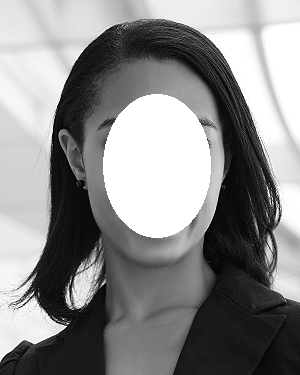
\includegraphics[width=1in,height=1.25in,clip,keepaspectratio]{a1.png}}]
{FIRST A. AUTHOR}~(Fellow, IEEE)~and all authors may include biographies.
Biographies are often not included in conference-related papers. This author
is an IEEE Fellow. The first paragraph may contain a place and/or date of
birth (list place, then date). Next, the author's educational background is
listed. The degrees should be listed with type of degree in what field,
which institution, city, state, and country, and year the degree was earned.
The author's major field of study should be lower-cased.

The second paragraph uses the pronoun of the person (he or she) and not the
author's last name. It lists military and work experience, including summer
and fellowship jobs. Job titles are capitalized. The current job must have a
location; previous positions may be listed without one. Information
concerning previous publications may be included. Try not to list more than
three books or published articles. The format for listing publishers of a
book within the biography is: title of book (publisher name, year) similar
to a reference. Current and previous research interests end the paragraph.

The third paragraph begins with the author's title and last name
(e.g., Dr.\ Smith, Prof.\ Jones, Mr.\ Kajor, Ms.\ Hunter). List any memberships in
professional societies other than the IEEE. Finally, list any awards and
work for IEEE committees and publications. If a photograph is provided, it
should be of good quality, and professional-looking.
\end{IEEEbiography}


\begin{IEEEbiographynophoto}
{SECOND B. AUTHOR,} photograph and biography not available at the time
of publication.
\end{IEEEbiographynophoto}


\begin{IEEEbiographynophoto}
{THIRD C. AUTHOR JR.}~(Member, IEEE), photograph and biography not available
at the time of publication.
\end{IEEEbiographynophoto}

\vfill\pagebreak

\end{document}
